\label{ch:anexos}
\chapter{Anexos}

\section{Diagrama de clases para el anotador}
\label{sec:diagramaClass}
\begin{figure}[H]
	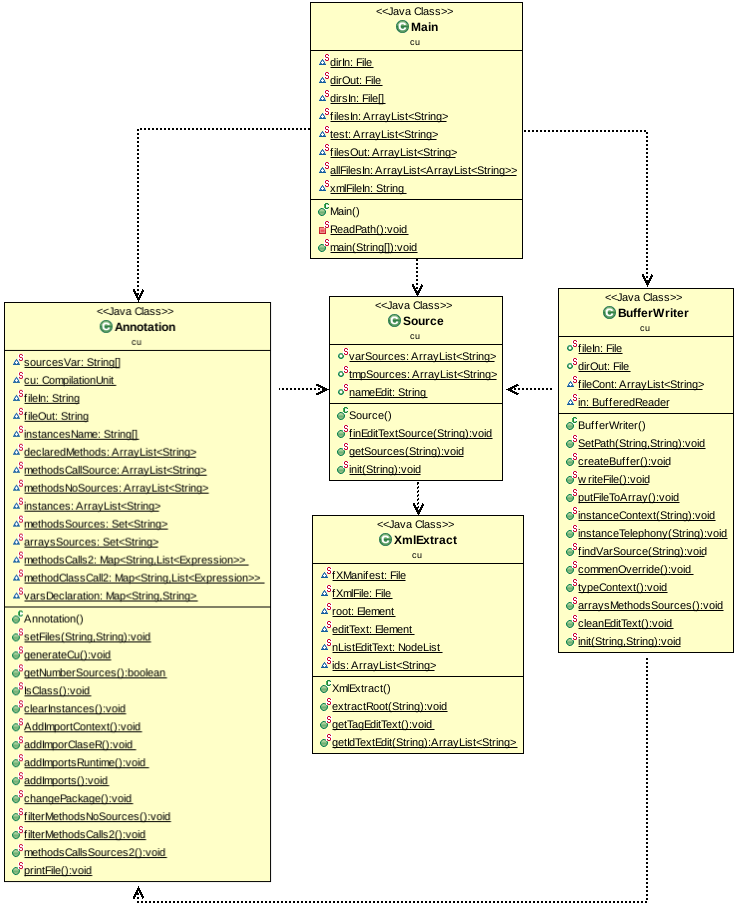
\includegraphics[width=13cm]{consolidado.png}
	\caption{Clases necesarias para la implementación del anotador}
	\label{fig:classDiagram} 
\end{figure}

\section{Descripción de testcases para evaluación}
\label{tb:muestra-descripApps}
\label{sec:testcases}
En las tablas \ref{tab:descripApps1}, \ref{tab:descripApps2} y
\ref{tab:descripApps3}, se describe el comportamiento de los casos de prueba
evaluados, donde:\newline 
Se considera con nivel de seguridad alto, variables y métodos que almacenan y
modifican(respectivamente), información catalogada como privada(Sources).\newline 
Se considera con nivel de seguridad bajo, métodos para envío de mensajes y para
muestra de logs.

En los casos en que se requiere, se precisan observaciones entre los
resultados de evaluación esperados para la técnica de análisis utilizada por
FlowDroid y la técnica de análisis propuesta en el presente trabajo.

\begin{table}[H]
\small\addtolength{\tabcolsep}{-3pt}
\caption{Descripción aplicaciones de prueba}
\label{tab:descripApps1}
\begin{tabular}{|p{13cm}|p{1cm}|}
	\hline
	\multicolumn{2}{|>{\columncolor[gray]{0.8}}c|}{\textbf{AndroidSpecific\_DirectLeak1}}\\
	\hline
	\textbf{Descripción} & \textbf{Leaks}\\
	\hline
	La variable \textit{mrg} tiene un nivel de seguridad alto,
	almacena información retornada por el método source \textit{getDeviceId}. Se
	genera flujo de información directo entre información con nivel de seguridad alto e
	información con nivel de seguridad bajo, al enviar como parámetro del método
	\textit{sendTextMessage}, información de la variable \textit{mrg}. & 1 \\
	\hline
	\multicolumn{2}{|>{\columncolor[gray]{0.8}}c|}{\textbf{AndroidSpecific\_InactiveActivity}}\\
	\hline
	\textbf{Descripción} & \textbf{Leaks}\\
	\hline 
	La variable \textit{imei} tiene un nivel de seguridad alto, almacena
	información retornada por el source getDeviceId. La variable es enviada como
	parámetro a \textit{Log}, canal que muestra información con nivel de
	seguridad bajo. \textit{Observación:} debido a que la actividad en que se
	presenta este flujo de información no está activada en el Manifest de la
	aplicación, para la técnica de análisis de FlowDroid no existen leaks. Para
	nuestra propuesta de análisis si existe leak, porque se asume que los métodos y
	sus aplicaciones podrán ser ejecutados. & 0
	\\
	\hline
	\multicolumn{2}{|>{\columncolor[gray]{0.8}}c|}{\textbf{AndroidSpecific\_LogNoLeak}}\\
	\hline
	\textbf{Descripción} & \textbf{Leaks}\\
	\hline
	El caso de prueba no presenta información con niveles de seguridad alto. Se
	presentan flujos de información entre información con el mismo nivel de
	seguridad, en este caso bajo, lo cual es permitido. & 0 \\
	\hline
	\multicolumn{2}{|>{\columncolor[gray]{0.8}}c|}{\textbf{AndroidSpecific\_Obfuscation1}}\\
	\hline
	\textbf{Descripción} & \textbf{Leaks}\\
	\hline 
	La variable \textit{\textbf{mrg}} tiene un nivel de seguridad alto,
	almacena información retornada por el método source getDeviceId().
	Se genera flujo de información entre información con nivel de seguridad alto e
	información con nivel de seguridad bajo, al enviar como parámetro del método
	\textit{sendTextMessage}, información de la variable
	\textit{mrg}. \textit{Observación:} el elemento adicional para este
	testcase es proveer una suplantación de la clase
	android.telephony.TelephonyManager, en el apk de la aplicación. Para la
	evaluación que proponemos, se verifica acorde a la versión que se tiene anotada
	para esta clase, es decir, independientemente de la ofuscación de la clase,
	nuestro análisis debe detectar que existe un flujo de información indebido. &
	1\\
	\hline
	\multicolumn{2}{|>{\columncolor[gray]{0.8}}c|}{\textbf{AndroidSpecific\_PrivateDataLeak2}}\\
	\hline
	\textbf{Descripción} & \textbf{Leaks}\\
	\hline
	La variable \textit{info} tiene un nivel de seguridad alto, almacena
	información suministrada por el campo EditText de tipo textPassword. Se genera
	flujo de información entre información con nivel de seguridad alto e
	información con nivel de seguridad bajo, al pasar la variable
	\textit{info} como parámetro de \textit{Log}, que muestra
	información con nivel de seguridad bajo. & 1 
	\\
	\hline
	\multicolumn{2}{|>{\columncolor[gray]{0.8}}c|}{\textbf{ArraysAndLists\_ArrayAccess1}}\\
	\hline
	\textbf{Descripción} & \textbf{Leaks}\\
	\hline
	Se tiene un array en que se almacena información tanto proveniente como no
	proveniente de sources, parte de la información que almacena es enviada como
	parámetro del método \textit{sendTextMessage}. \textit{Observación:}
	Para la técnica de análisis de FlowDroid(taint analysis), se marca únicamente el
	índice del array donde se almacena el dato considerado como source, así,
	cuando se envía como parámetro del método \textit{sendTextMessage},
	el dato de un índice no marcado, no se genera leak. Para nuestra técnica
	de análisis(flujo de información mediante JIF), para que un array almacene
	información con nivel de seguridad alto, primero debe ser catalogo(anotado)
	con nivel de seguridad alto, lo que implica que el array podrá almacenar
	información tanto de nivel de seguridad alto como bajo, pero toda la
	información quedará con nivel de seguridad alto. En consecuencia, al enviar
	cualquier índice del array como parámetro del método 
	\textit{sendTextMessage} se presenta un flujo de información no
	permitido. & 0
	\\
	\hline
\end{tabular}
\end{table}

\begin{table}[H]
\small\addtolength{\tabcolsep}{-3pt}
\caption{Descripción aplicaciones de prueba}
\label{tab:descripApps2}
\begin{tabular}{|p{13cm}|p{1cm}|}
	\hline
	\multicolumn{2}{|>{\columncolor[gray]{0.8}}c|}{\textbf{ArraysAndLists\_ArrayAccess2}}\\
	\hline
	\textbf{Descripción} & \textbf{Leaks}\\
	\hline
	Se presenta el contexto descrito en ArraysAndLists\_ArrayAccess1, con un
	elemento adicional, se implementa el método calculateIndex(), que calcula el
	índice del array a ser enviado como parámetro del método
	\textit{sendTextMessage}. & 0 \\
	\hline
	\multicolumn{2}{|>{\columncolor[gray]{0.8}}c|}{\textbf{GeneralJava\_Exceptions1}}\\
	\hline
	\textbf{Descripción} & \textbf{Leaks}\\
	\hline
	La variable \textit{imei} es de nivel de seguridad alto, almacena información
	devuelta por el método \textit{getDeviceId}. Se genera flujo de información
	entre información de nivel de seguridad alto e información con nivel de
	seguridad bajo, al enviar como parámetro del método \textit{sendTextMessage}
	información de la variable \textit{imei}. Este flujo de información se presenta
	dentro de la captura de una excepción RuntimeException(no es verificada
	en tiempo de compilación).
	& 1
	\\
	\hline
	\multicolumn{2}{|>{\columncolor[gray]{0.8}}c|}{\textbf{GeneralJava\_Exceptions2}}\\
	\hline
	\textbf{Descripción} & \textbf{Leaks}\\
	\hline
	La variable \textit{imei} es de nivel de seguridad alto, almacena información
	devuelta por el método \textit{getDeviceId}. El control de flujo del
	programa conduce de manera implícita a la captura de una excepción tipo
	RuntimeException, desde allí se utiliza información proveída por la variable
	\textit{imei}, como parámetro para invocar el método \textit{sendTextMessage}.
	Generando un flujo de información indebido. & 1
	\\
	\hline
	\multicolumn{2}{|>{\columncolor[gray]{0.8}}c|}{\textbf{GeneralJava\_Exceptions3}}\\
	\hline
	\textbf{Descripción} & \textbf{Leaks}\\
	\hline
	La variable \textit{imei} es de nivel de seguridad alto, almacena información
	devuelta por el método \textit{getDeviceId}. La información proveída por
	\textit{imei} es utilizada como parámetro para invocar el método
	\textit{sendTextMessage} dentro de la captura de una excepción tipo
	RuntimeException, sin embargo, el programa no genera un caso que haga ejecutar
	la captura de la excepción. & 0
	\\
	\hline
	\multicolumn{2}{|>{\columncolor[gray]{0.8}}c|}{\textbf{GeneralJava\_Exceptions4}}\\
	\hline
	\textbf{Descripción} & \textbf{Leaks}\\
	\hline
	La variable \textit{imei} es de nivel de seguridad alto, almacena información
	devuelta por el método \textit{getDeviceId}. información proveída por esta
	variable es enviada como parámetro para la captura de una excepción en tiempo
	de ejecución, donde es utilizado como parámetro para invocar el método
	\textit{sendTextMessage}, generando un flujo de información indebido. & 1\\
	\hline
	\multicolumn{2}{|>{\columncolor[gray]{0.8}}c|}{\textbf{GeneralJava\_Loop1}}\\
	\hline
	\textbf{Descripción} & \textbf{Leaks}\\
	\hline
	La variable \textit{imei} es de nivel de seguridad alto, almacena información
	devuelta por el método \textit{getDeviceId}. Se generan flujos de información
	indebidos, primero al tratar de asignar la información de la variable a un
	array con nivel de seguridad bajo(donde se intenta ofuscar la información),
	luego al tratar de enviar la información ofuscada como parámetro del método
	\textit{sendTextMessage}, con nivel de seguridad bajo. & 1 \\
	\hline
	\multicolumn{2}{|>{\columncolor[gray]{0.8}}c|}{\textbf{GeneralJava\_Loop2}}\\
	\hline
	\textbf{Descripción} & \textbf{Leaks}\\
	\hline
	La variable \textit{imei} es de nivel de seguridad alto, almacena información
	devuelta por el método \textit{getDeviceId}. Se busca ofuscar la información de
	\textit{imei} mediante ciclos for anidados, allí se asigna la información de la
	variable a un array con nivel de seguridad bajo. Luego se envía la información
	ofuscada, como parámetro del método \textit{sendTextMessage}, con nivel de
	seguridad bajo, generando otro flujo de información indebido. & 1\\
	\hline
\end{tabular}
\end{table}

\begin{table}[H]
\small\addtolength{\tabcolsep}{-3pt}
\caption{Descripción aplicaciones de prueba}
\label{tab:descripApps3}
\begin{tabular}{|p{13cm}|p{1cm}|}
	\multicolumn{2}{|>{\columncolor[gray]{0.8}}c|}{\textbf{GeneralJava\_UnreachableCode}}\\
	\hline
	\textbf{Descripción} & \textbf{Leaks}\\
	\hline
	La variable \textit{deviceid} con nivel de seguridad alto, está contenida en un
	método que no es llamado, dentro del mismo, \textit{deviceid} es pasada como
	parámetro para invocar el método \textit{sendTextMessage}, cuyo nivel de
	seguridad es bajo. \textit{Observaciones:} para el análisis de FlowDroid el
	programa no presenta leaks, ya que el método nunca es llamado.
	Para nuestro análisis, el programa presenta leak porque se asume que todos los
	métodos son llamados. & 0\\
	\hline
	\multicolumn{2}{|>{\columncolor[gray]{0.8}}c|}{\textbf{ImplicitFlows\_ImplicitFlow1}}\\
	\hline
	\textbf{Descripción} & \textbf{Leaks}\\
	\hline
	 La variable \textit{imei} con nivel de seguridad alto, almacena información
	 devuelta por el método \textit{getDeviceId}, \textit{imei} se pasa como
	 parámetro al método obfuscateIMEI que devuelve la información ofuscada.
	 Después se invoca el método WriteToLog, con la información ofuscada como
	 parámetro para ser mostrada en el log. Al invocar el método WriteToLog con la
	 información ofuscada, se genera un flujo de información indebido. & 1 \\
	\hline
	\multicolumn{2}{|>{\columncolor[gray]{0.8}}c|}{\textbf{ImplicitFlows\_ImplicitFlow2}}\\
	\hline
	\textbf{Descripción} & \textbf{Leaks}\\
	\hline
	 La variable \textit{userInputPassword} con nivel de seguridad alto, almacena
	 información de un campo EditText tipo textPassword(password suministrado por
	 el usuario). Se generan flujos de información indebidos: al tratar de asignar
	 información a la variable passwordCorrect con nivel de seguridad bajo, a
	 partir de la comparación de información con nivel de seguridad alto(variable
	 textPassword), después, al tratar de mostrar en el \textit{log} información
	 que depende de tal comparación. & 1\\
	\hline
	\multicolumn{2}{|>{\columncolor[gray]{0.8}}c|}{\textbf{ImplicitFlows\_ImplicitFlow4}}\\
	\hline
	\textbf{Descripción} & \textbf{Leaks}\\
	\hline
	La variable \textit{password} con nivel de seguridad alto, almacena información
	de un campo EditText tipo textPassword, \textit{password} es utilizada como
	parte de los parámetros para invocar el método \textit{lookup} que busca
	identificar el password suministrado por el usuario. Se genera un flujo de
	información indebido, cuando se compara lo retornado por el método para mostrar
	en el \textit{log} información del password. & 1 \\
	\hline
	\multicolumn{2}{|>{\columncolor[gray]{0.8}}c|}{\textbf{Lifecycle\_ActivityLifecycle3}}\\
	\hline
	\textbf{Descripción} & \textbf{Leaks}\\
	\hline
	 El flujo de información entre información con nivel de seguridad alto e
	 información con nivel de seguridad bajo, tiene lugar a través de dos
	 métodos del ciclo de vida de la actividad: onSaveInstanceState y
	 onRestoreInstanceState. En onSaveInstanceState, se asigna información con
	 nivel de seguridad alto a la variable \textit{s}, la información que almacene
	 este método es utilizada durante la reanudación de la actividad, a través del
	 método onRestoreInstanceState, donde se muestra en el \textit{log} información
	 de la variable \textit{s}. & 1\\
	\hline
	\multicolumn{2}{|>{\columncolor[gray]{0.8}}c|}{\textbf{Lifecycle\_BroadcastReceiverLifecycle1}}\\
	\hline
	\textbf{Descripción} & \textbf{Leaks}\\
	\hline
	 Se tiene un broadcast receiver  que muestra información con nivel de
	 seguridad alto, contenida en la variable \textit{imei}(almacena información retornada por el
	 método \textit{getDeviceId}) a través del \textit{log}. & 1 \\
	\hline
	\multicolumn{2}{|>{\columncolor[gray]{0.8}}c|}{\textbf{Lifecycle\_ServiceLifecycle1}}\\
	\hline
	\textbf{Descripción} & \textbf{Leaks}\\
	\hline
	 Se tiene un servicio que presenta flujo de información indebida mediante dos
	 métodos de su ciclo de vida. En el método que inicia el servicio
	 onStartCommand, la variable con nivel de seguridad alto, almacena
	 información devuelta por el método \textit{getDeviceId}. Luego el método
	 onLowMemory, se envía información de la variable \textit{secret} a través de
	 un mensaje msm. & 1\\
	\hline
\end{tabular}
\end{table}

% \section{Formulas}
% Las formulas \ref{p} y \ref{r} son aplicadas para calcular los porcentajes
% de Precisión(p) y Recall(r).
% \begin{equation}
% \label{p}
% 	p = TP/(TP +FP) 
% \end{equation}
% \begin{equation}
% \label{r}
% 	r = TP/(TP+FN)
% \end{equation}
% 
% Donde: \newline
% TP representa el total de verdaderos positivos; FP corresponde al total de
% falsos positivos y  FN representa el total de falsos
% negativos; reportados por la herramienta.\newline

\section{Instrucciones para probar el prototipo}
\label{sec:ejecutarPrototipo}
En el directorio \small{\ttfamily{/home/testing/eule}} están los elementos
necesarios para evaluar los casos de prueba, de allí interesan los
subdirectorios \small{\ttfamily{androidFlows}},
\small{\ttfamily{InputLabelGenerator}} y el jar
\small{\ttfamily{LabelGenerator.jar}}.

El subdirectorio \small{\ttfamily{androidFlows}} contiene la estructura de
archivos necesaria para ejecutar un programa jif, así:
\small{\ttfamily{sig-src}} aloja clases java y clases de la API de Android, con
signaturas para que jif las reconozca de forma nativa.
\small{\ttfamily{jif-src/test}} tiene clases de la API de Android con
anotaciones jif(Activity.jif, BroadcastReceiver.jif, Log.jif, R.jif,
Service.jif, SmsManager.jif). Allí se deben alojar los programas jif a
ejecutar.\newline 
En {\small{\ttfamily{InputLabelGenerator}}} están los fuentes java a pasar como
entrada para el generador de labels(LabelGenerator.jar), que devuelve la
versión jif de los mismos. Se recomienda utilizar estos, ya que contienen las
adaptaciones necesarias para poder ser analizadas con JIF, la adición de
excepciones NullPointerException, ClassCastException y
ArrayIndexOutOfBoundsException, son algunos ejemplos de elementos adicionados.

 \textbf{Instrucciones de
ejecución:}\newline \textbf{(1)} Ejecutar el jar para la generación de los labels:
\begin{lstlisting}
testing@debianJessie:~/eule$ java -jar LabelGenerator.jar
\end{lstlisting}
Una vez se ejecuta el .jar, se solicita el directorio de entrada(que contiene
las aplicaciones a anotar) y el directorio de salida(para alojar las
aplicaciones anotadas). Separados por el simbolo @
\begin{lstlisting}
Ingrese la ruta completa para el directorio de entrada, y para el 
directorio de salida:
Ejemplo: dir-entrada@dir-salida 
\end{lstlisting}
Se deben pasar los directorios:
\begin{lstlisting}
InputLabelGenerator@androidFlows/jif-src/test/
\end{lstlisting}

\textbf{(2)} ejecutar el script setup.sh(basta con ejecutarlo una sola vez)
\begin{lstlisting}
testing@debianJessie:~/eule/androidFlows$ ./setup.sh
\end{lstlisting}

\textbf{(3)} 
Ejecutar el .jif generado:\newline
En la ruta pasada como directorio de salida en el punto anterior
{\small{\ttfamily{androidFlows/jif-src/test}}}, se genera un subdirectorio por
aplicación, con un .java y un *-out.jif. Se debe ejecutar el *-out.jif. Por
ejemplo, para evaluar el testcase ArraysAndLists\_ArrayAccess1:
\begin{lstlisting}
testing@debianJessie:~/eule/androidFlows$ ./jifc-java-libraries.sh \
jif-src/test/ArraysAndLists_ArrayAccess1/ArrayAccess1-out.jif
\end{lstlisting}
Cuando se presentan flujos indebidos, el compilador genera una salida señalando
los problemas de seguridad.
\lstset{
    language=bash,
    basicstyle=\tiny,
  }
\begin{lstlisting}
estudiante@debianJessie:~/eule/androidFlows$ ./jifc-java-libraries.sh \
jif-src/test/ArraysAndLists_ArrayAccess1/ArrayAccess1-out.jif 
/home/testing/eule/androidFlows/jif-src/test/ArraysAndLists_ArrayAccess1/ArrayAccess1-out.jif:51:
Unsatisfiable constraint
    	general constraint:
    		actual_arg_3 <= formal_arg_3
    	in this context:
    		{Alice->; _<-_ ⊔ caller_pc} <= {}
    	cannot satisfy equation:
    		{Alice->} ⊑ {}
    	in environment:
    		{this} ⊑ {caller_pc}
    		[]

    Label Descriptions
    ------------------
     - actual_arg_3 = the label of the 3rd actual argument
     - actual_arg_3 = {Alice->; _<-_ ⊔ caller_pc}
     - formal_arg_3 = the upper bound of the formal argument text
     - formal_arg_3 = {}
     - caller_pc = The pc at the call site of this method (bounded above by 
    {})
     - this = label of the special variable "this" in test.ArrayAccess1

    The label of the actual argument, actual_arg_3, is more restrictive than 
    the label of the formal argument, formal_arg_3.
            sms.sendTextMessage("+49 1234", null, arrayData[2], null, null);
                                                  ^-------^

1 error.
testing@debianJessie:~/eule/androidFlows$
\end{lstlisting}

Cuando el caso de prueba no presenta flujos indebidos, el compilador no genera
salidas, por ejemplo, al evaluar el testcase AndroidSpecific\_LogNoLeak, el
compilador retorna el prompt de la shell, sin ningún comentario.

\section{Instrucciones para uso de FlowDroid}
En el directorio \small{\ttfamily{/home/estudiante/eule}} también se encuentran
los subdirectorios \small{\ttfamily{/FlowDroid}} y
\small{\ttfamily{/DroidBench-master}} que contienen los elementos necesarios
para probar los testcases con FlowDroid.\newline 
Para ello se requiere ejecutar el jar de FlowDroid, indicando el apk a analizar,
los apk están en el subdirectorio \tetxtit{DroidBench-master}.
Por ejemplo, para analizar el testace ImplicitFlow4:
\begin{lstlisting}
testing@debianJessie:~/eule/FlowDroid$ java -jar FlowDroid.jar \
../DroidBench-master/apk/ImplicitFlows/ImplicitFlow4.apk
/home/estudiante/android-sdks/platforms/
\end{lstlisting}
El archivo \small{\ttfamily{howRunIt}} contenido en el directorio
\small{\ttfamily{/FlowDroid}}, indica como se debe ejecutar.